% Created 2017-04-11 Tue 16:57
% Intended LaTeX compiler: pdflatex
\documentclass[presentation,10pt]{beamer}
\usepackage[utf8]{inputenc}
\usepackage[T1]{fontenc}
\usepackage{graphicx}
\usepackage{grffile}
\usepackage{longtable}
\usepackage{wrapfig}
\usepackage{rotating}
\usepackage[normalem]{ulem}
\usepackage{amsmath}
\usepackage{textcomp}
\usepackage{amssymb}
\usepackage{capt-of}
\usepackage{hyperref}
\usepackage{amsthm}
\usepackage{amsmath}
\usepackage{amssymb}
\usepackage{mathtools}
\newtheorem{mydef}{Definition}
\newtheorem{mythm}{Theorem}
\newcommand{\dx}{\mathrm{d}}
\newcommand{\var}{\mathrm{var}}
\newcommand{\cov}{\mathrm{cov}}
\newcommand{\corr}{\mathrm{corr}}
\newcommand{\pr}{\mathrm{Pr}}
\newcommand{\rarrowd}[1]{\xrightarrow{\text{ \textit #1 }}}
\DeclareMathOperator*{\plim}{plim}
\newcommand{\plimn}{\plim_{n \rightarrow \infty}}
\usepackage{booktabs}
\usepackage{color}
\usepackage{caption}
\usepackage{subcaption}
\def\mathbi#1{\textbf{\em #1}}
\usetheme{CambridgeUS}
\usecolortheme{beaver}
\author{Zheng Tian}
\date{}
\title{Lecture 8: Linear Regression with Multiple Regressors}
\hypersetup{
 pdfauthor={Zheng Tian},
 pdftitle={Lecture 8: Linear Regression with Multiple Regressors},
 pdfkeywords={},
 pdfsubject={},
 pdfcreator={Emacs 25.1.1 (Org mode 9.0.3)}, 
 pdflang={English}}
\begin{document}

\maketitle
\begin{frame}{Outline}
\setcounter{tocdepth}{1}
\tableofcontents
\end{frame}



\section{The Multiple Regression Model}
\label{sec:org6e63a3b}
\setcounter{tocdepth}{1}
\tableofcontents[currentsection]

\begin{frame}[label={sec:orgd601ec5}]{The problem of a simple linear regression}
\begin{block}{The simple linear regression model}
\begin{equation*}
TestScore = \beta_0 + \beta_1 \times STR + OtherFactors
\end{equation*}
\end{block}

\begin{block}{Question: Is this model adequate to characterize the determination of test scores?}
\begin{itemize}
\item It ignores many important factors, simply lumped into
\emph{OtherFactors}, the error term, \(u_i\), in the regression model.

\item What are possible other important factors?
\begin{itemize}
\item School district characteristics: average income level, demographic
components
\item School characteristics: teachers' quality, school buildings,
\item Student characteristics: family economic conditions, individual
ability
\end{itemize}
\end{itemize}
\end{block}
\end{frame}

\begin{frame}[label={sec:org86d5e73}]{Percentage of English learners as an example}
The percentage of English learners in a school district could be an
relevant and important determinant of test scores, which is omitted
in the simple regression model.

\begin{block}{How can it affect the estimate of the effect of student-teacher ratios on test score?}
\begin{itemize}
\item High percentage of English learners \(\Rightarrow\) large student-teacher ratios.

\item High percentage of English learners \(\Rightarrow\) lower test scores.

\item The estimated effect of student-teacher ratios may in fact include
the influence from the high percentage of English learners.

\item In the terminology of statistics, the magnitude of the coefficient
on student-teacher ratio is \alert{overestimated}.

\item The problem is called \alert{the omitted variable bias}
\end{itemize}
\end{block}
\end{frame}

\begin{frame}[label={sec:org8940ab9}]{Solutions to the problem of ignoring important factors}
We can include these important but ignored variables, like the
percentage of English learners (\(PctEL\)), in the regression model.  

\[
TestScore_i = \beta_0 + \beta_1 STR_i + \beta_2 PctEL_i +
OtherFactors_i 
\] 

A regression model with more than one regressors is a multiple
regression model. 
\end{frame}

\begin{frame}[label={sec:orgffd2cdb}]{A multiple regression model}
The general form of a \alert{multiple regression model} is
\begin{equation}
\label{eq:multi-regress-1}
Y_i = \beta_0 + \beta_1 X_{1i} + \beta_2 X_{2i} + \cdots + \beta_k X_{ki} + u_i,\; i = 1, \ldots, n
\end{equation}
where
\begin{itemize}
\item \(Y_i\) is the i\(^{\text{th}}\) observation on the dependent variable;
\item \(X_{1i}, X_{2i}, \ldots, X_{ki}\) are the i\(^{\text{th}}\) observation on each
of the \(k\) regressors; and
\item \(u_i\) is the error term associated with the i\(^{\text{th}}\) observation,
representing all other factors that are not included in the model.
\end{itemize}
\end{frame}

\begin{frame}[label={sec:orge67f546}]{The components in a multiple regression model}
\begin{itemize}
\item The population regression line (or population regression
function)
\begin{equation*}
E(Y_i | X_{1i}, \ldots, X_{ki}) = \beta_0 + \beta_1 X_{1i} + \cdots + \beta_k X_{ki}
\end{equation*}

\item \(\beta_1, \ldots, \beta_k\) are the coefficients on the corresponding
\(X_i,\, i = 1, \ldots, k\).

\item \(\beta_0\) is the intercept, which can also be thought of the
coefficient on a regressor \(X_{0}\) that equals 1 for all
observations.

\begin{itemize}
\item Including \(X_{0}\), there are \(k+1\) regressors in the multiple
regression model.
\end{itemize}
\end{itemize}
\end{frame}

\begin{frame}[label={sec:orga14b840}]{The interpretation of \(\beta_i\): Holding other things constant}
\begin{equation}
\label{eq:multi-regress-1a}
Y = \beta_0 + \beta_1 X_1 + \cdots + \beta_k X_k + u
\end{equation}

The coefficient \(\beta_i\) on the regressor
\(X_i\) for \(i=1, \ldots, k\) measures the effect on \(Y\) of a unit change
in \(X_i\), \alert{holding other \(X\) constant}. 

\begin{block}{An example}
Suppose we have two regressors \(X_1\) and \(X_2\) and we are interested
in the effect of \(X_1\) on \(Y\). We can let \(X_1\) change by \(\Delta X_1\)
and holding \(X_2\) constant. Then, the new value of \(Y\) is

\[ Y + \Delta Y = \beta_0 + \beta_1 (X_1 + \Delta X_1) + \beta_2 X_2  \]

Subtracting \(Y = \beta_0 + \beta_1 X_1 + \beta_2 X_2\), we have
\(\Delta Y = \beta_1 \Delta X_1\). That is
\[ \beta_1 = \frac{\Delta Y}{\Delta X}, \text{ holding } X_2 \text{ constant} \]
\end{block}
\end{frame}

\begin{frame}[label={sec:orgebb42e8}]{The partial effect}
If \(Y\) and \(X_i\) for \(i = 1, \ldots, k\) are continuous and
differentiable variables, \(\beta_i\) is as simply as the partial
derivative of \(Y\) with respect to \(X_i\). That is

\[\beta_i = \frac{\partial Y}{\partial X_i}\]

By the definition of a partial derivative, \(\beta_i\) is just
the effect of a marginal change in \(X_i\) on \(Y\) holding other \(X\)
constant.
\end{frame}

\begin{frame}[label={sec:org8778c85}]{Look at the data in terms of vectors and matrix}
\begin{figure}[htbp]
\centering
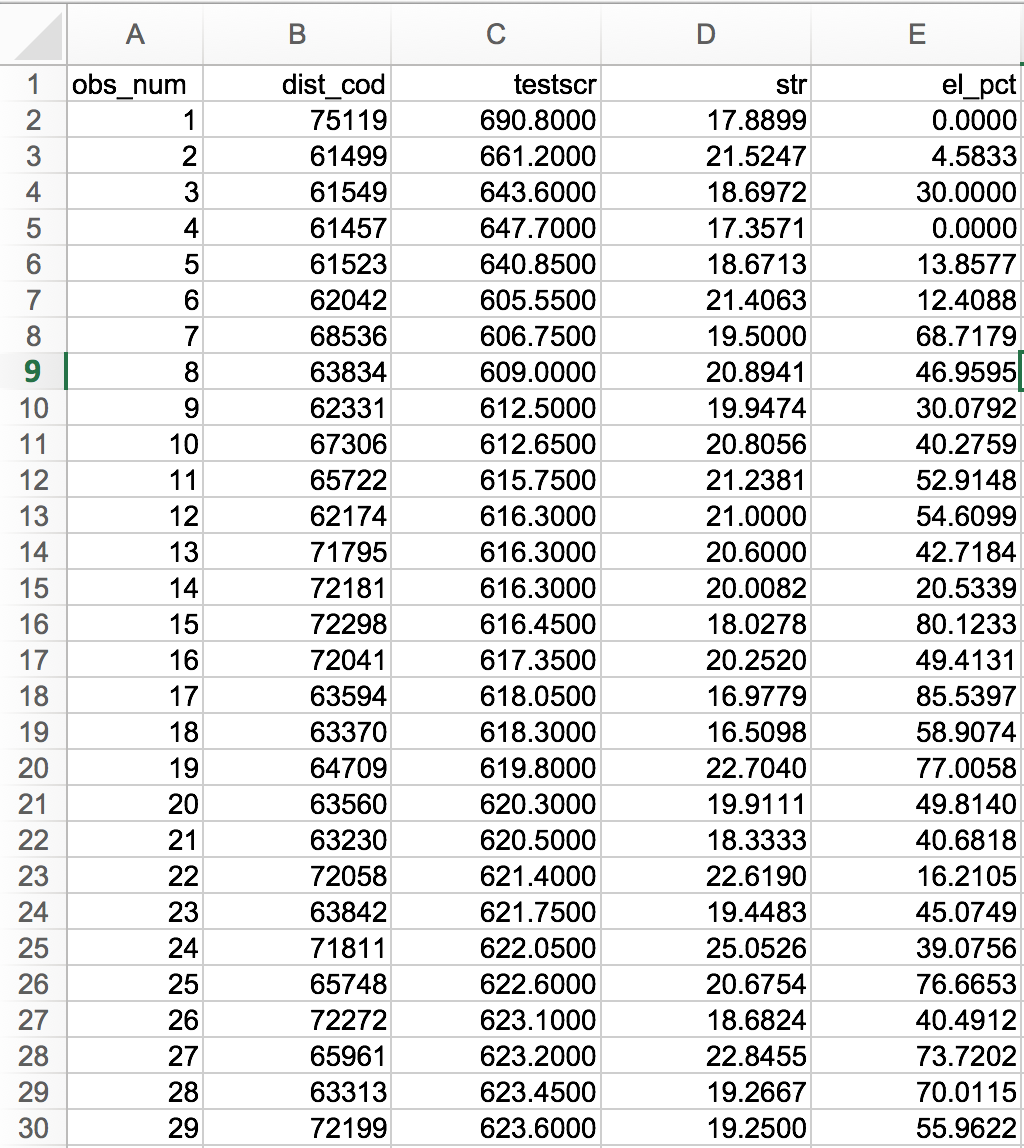
\includegraphics[width=0.4\textwidth,height=0.5\textheight]{img/data_snapshot.png}
\caption{\label{fig:org8b6563b}
The California data set in Excel}
\end{figure}

\begin{itemize}
\item Each row represents an observation of all variables pertaining to a
school district.
\item Each column represents a variable with all
observations.
\item The whole dataset can be seen as a matrix.
\end{itemize}
\end{frame}

\begin{frame}[shrink,label={sec:org8c739a2}]{Define variables in matrix notation}
\begin{block}{Write all the variables in vector and matrix notation}
\begin{equation*}
\underbrace{
\mathbf{Y} =
\begin{pmatrix}
Y_1 \\
Y_2 \\
\vdots \\
Y_n
\end{pmatrix},}_{\text{Dependent variable}}
\underbrace{
\mathbf{X} =
\begin{pmatrix}
1 & X_{11} & \cdots & X_{k1} \\
1 & X_{12} & \cdots & X_{k2} \\
\vdots & \vdots & \ddots & \vdots \\
1 & X_{1n} & \cdots & X_{kn}
\end{pmatrix},}_{\text{Independent variables}}
\underbrace{
\mathbf{u} =
\begin{pmatrix}
u_1 \\
u_2 \\
\vdots \\
u_n
\end{pmatrix},\,}_{\text{Errors}}
\underbrace{
\boldsymbol{\beta} =
\begin{pmatrix}
\beta_0 \\
\beta_1 \\
\vdots \\
\beta_k
\end{pmatrix}}_{\text{Coefficients}}
\end{equation*}
\end{block}

\begin{block}{Write the multiple regression model in matrix notation}
\begin{equation}
\label{eq:multi-regress-m}
\mathbf{Y} = \mathbf{X} \boldsymbol{\beta} + \mathbf{u}
\end{equation}
\end{block}

\begin{block}{Why do we use matrix notation}
Concise, easy to derive properties; big-picture perspective.
\end{block}
\end{frame}


\begin{frame}[label={sec:org1b0f6ad}]{Two other ways to write the regression model}
\begin{block}{Write \(\mathrm{X}\) in row vectors}
\begin{itemize}
\item The i\(^{\text{th}}\) row in \(\mathrm{X}\) is a \((k+1) \times 1\) vector
\begin{equation*}
\mathbi{x}_i =
\begin{pmatrix}
1 \\
X_{1i} \\
\vdots \\
X_{ki} \\
\end{pmatrix}. \text{ Thus, its transpose is }
\mathbi{x}_i^{\prime} = (1, X_{1i}, \cdots, X_{ki})
\end{equation*}

\item We can write the regression model (Equation
\ref{eq:multi-regress-m}) as

\begin{equation}
Y_i = \mathbi{x}^{\prime}_i \boldsymbol{\beta} + u_i,\; i = 1, \ldots, n
\end{equation}
\end{itemize}
\end{block}
\end{frame}

\begin{frame}[label={sec:orgdc768e6}]{Two other ways to write the regression model (cont'd)}
\begin{block}{Write \(\mathrm{X}\) in vector vectors}
\begin{itemize}
\item The i\(^{\text{th}}\) column in \(\mathbf{X}\) is a \(n \times 1\) vector
\begin{equation*}
\boldsymbol{X}_i =
\begin{pmatrix}
X_{i1} \\
\vdots \\
X_{in} \\
\end{pmatrix}. \text{ The first column is }
\boldsymbol{\iota} = 
\begin{pmatrix}
1 \\
\vdots \\
1
\end{pmatrix}. \text{ Thus }
\mathbf{X} = \left(\boldsymbol{\iota}, \boldsymbol{X}_1, \ldots, \boldsymbol{X}_k \right)
\end{equation*}

\item The regression model (Equation \ref{eq:multi-regress-m}) can be
re-written as
\begin{equation}
\label{eq:multi-regress-m2}
\mathbf{Y} = \beta_0 \boldsymbol{\iota} + \beta_1\boldsymbol{X}_1 + \cdots + \beta_k\boldsymbol{X}_k + \mathbf{u}
\end{equation}
\end{itemize}
\end{block}
\end{frame}


\section{The OLS Estimator in Multiple Regression}
\label{sec:org0426ff4}
\setcounter{tocdepth}{1}
\tableofcontents[currentsection]

\begin{frame}[label={sec:orgd435edd}]{The minimization problem and the OLS estimator}
\begin{itemize}
\item The core idea of the OLS estimator for a multiple regression model
remains the same as in a simple regression model: 
\alert{minimizing the sum of the squared residuals}.

\item Let \(\mathbf{b} = [b_0, b_1, \ldots, b_k]^{\prime}\) be some estimators
of \(\boldsymbol{\beta} = [\beta_0, \beta_1, \ldots,
  \beta_k]^{\prime}\).

\item The predicted \(Y_i\) is
\begin{gather*}
\hat{Y}_i = b_0 + b_1 X_{1i} + \cdots + b_k X_{ki} = \mathbi{x}^{\prime}_i
\mathbf{b},\, i = 1, \ldots, \\
\text{ or in matrix notation }  \hat{\mathbf{Y}} = \mathbf{Xb}
\end{gather*}

\item The residuals, i.e., the prediction mistakes, with \(\mathbf{b}\) is
\begin{gather*}
\hat{u}_i = Y_i - b_0 - b_1 X_{1i} - \cdots - b_k X_{ki} = Y_i -
\mathbi{x}^{\prime}_i \mathbf{b} \\
\text{ or in matrix notation }  \hat{\mathbf{u}} = \mathbf{Y} - \mathbf{Xb}
\end{gather*}
\end{itemize}
\end{frame}

\begin{frame}[label={sec:org9218b48}]{The minimization problem and the OLS estimator (cont'd)}
\begin{itemize}
\item The sum of the squared residuals is
\begin{align*}
S(\mathbf{b}) & = S(b_0, b_1, \ldots, b_k) = \sum_{i=1}^n (Y_i - b_0 - b_1 X_{1i} - \cdots - b_k X_{ki})^2 \\
& = \sum_{i=1}^n (Y_i - \mathbf{x}^{\prime}_i \mathbf{b})^2 = (\mathbf{Y} -
\mathbf{Xb})^{\prime}(\mathbf{Y}-\mathbf{Xb}) \\
& = \hat{\mathbf{u}}^{\prime} \hat{\mathbf{u}} = \sum_{i=1}^n \hat{u}_i^2
\end{align*}

\item The OLS estimator is the solution to the following minimization problem:
\begin{equation}
\label{eq:ols-multi-regress}
\operatorname*{min}_{\mathbf{b}}\: S(\mathbf{b}) = \hat{\mathbf{u}}^{\prime} \hat{\mathbf{u}}
\end{equation}
\end{itemize}
\end{frame}

\begin{frame}[label={sec:orga9e77ca}]{The OLS estimator of \(\boldsymbol{\beta}\) as a solution to the minimization problem}
\begin{itemize}
\item Solve the minimization problem: 

$$\text{F.O.C.: } \frac{\partial S(\mathbf{b})}{\partial b_j} = 0,
  \text{ for } j =
  0, 1, \ldots, k$$

\item The derivative of \(S(b_0, \ldots, b_k)\) with respect to \(b_j\) is
\begin{gather*}
\label{eq:ols-wrt-bj}
\frac{\partial }{\partial b_j} \sum_{i=1}^n \left(Y_i - b_0 - b_1 X_{1i} - \cdots - b_k X_{ki} \right)^2 = \\
-2 \sum_{i=1}^n X_{ji} \left(Y_i - b_0 - b_1 X_{1i} - \cdots - b_k X_{ki} \right) = 0
\end{gather*}

\item There are \(k+1\) such equations. Solving the system of equations, we
obtain the OLS estimator \(\hat{\boldsymbol{\beta}} = (\hat{\beta}_0, \ldots,
  \hat{\beta}_k)^{\prime}\).
\end{itemize}
\end{frame}

\begin{frame}[label={sec:orgc766047}]{The OLS estimator in matrix notation}
Let \(\boldsymbol{\hat{\beta}}\) denote the OLS estimator. Then the
expression of \(\boldsymbol{\hat{\beta}}\) is given by
\begin{equation}
\label{eq:betahat-mult}
\boldsymbol{\hat{\beta}} = (\mathbf{X}^{\prime} \mathbf{X})^{-1} \mathbf{X}^{\prime} \mathbf{Y}
\end{equation}

\begin{block}{Some useful results of matrix calculus}
To prove Equation (\ref{eq:betahat-mult}), we need to use some results
of matrix calculus.
\begin{equation}
\label{eq:matrix-calc}
\frac{\partial \mathbf{a}^{\prime} \mathbf{x}}{\partial \mathbf{x}} = \mathbf{a},\; \frac{\partial \mathbf{x}^{\prime} \mathbf{a}}{\partial \mathbf{x}} = \mathbf{a},\; \text{ and } \frac{\partial \mathbf{x}^{\prime} \mathbf{A} \mathbf{x}}{\partial \mathbf{x}} = (\mathbf{A} + \mathbf{A}^{\prime}) \mathbf{x}
\end{equation}
when \(\mathbf{A}\) is symmetric, then \((\partial \mathbf{x}^{\prime}
\mathbf{A} \mathbf{x}) / (\partial \mathbf{x}) = 2\mathbf{A}
\mathbf{x}\)
\end{block}
\end{frame}

\begin{frame}[label={sec:org6014bcb}]{The proof}
\begin{proof}[Proof of Equation (\ref{eq:betahat-mult})]
  \begin{equation*}
  S(\mathbf{b}) = \hat{\mathbf{u}}^{\prime} \hat{\mathbf{u}} = \mathbf{Y}^{\prime} \mathbf{Y} - \mathbf{b}^{\prime} \mathbf{X}^{\prime} \mathbf{Y} - \mathbf{Y}^{\prime} \mathbf{Xb} - \mathbf{b}^{\prime} \mathbf{X}^{\prime} \mathbf{Xb}
  \end{equation*}

  The first order conditions for minimizing $S(\mathbf{b})$ with respect to $\mathbf{b}$ is
  \begin{gather}
  -2 \mathbf{X}^{\prime} \mathbf{Y} - 2 \mathbf{X}^{\prime} \mathbf{Xb} = \mathbf{0} \notag \\
  \mathbf{X}^{\prime} \mathbf{Xb} = \mathbf{X}^{\prime} \mathbf{Y} \label{eq:ols-mult-eqs}
  \end{gather}

  Then
  \begin{equation*}
  \mathbf{b} = (\mathbf{X}^{\prime} \mathbf{X})^{-1} \mathbf{X}^{\prime} \mathbf{Y}
  \end{equation*}
  given that $\mathbf{X}^{\prime} \mathbf{X}$ is invertible.
\end{proof}

Note that Equation (\ref{eq:ols-mult-eqs}) represents a system of
equations with \(k+1\) equations.
\end{frame}

\begin{frame}[label={sec:org1befa41}]{The OLS estimator of \(\hat{\beta}_1\) in a simple regression model}
The simple linear regression model written in matrix notation is

\begin{equation*}
\mathbf{Y} = \beta_0 \boldsymbol{\iota} + \beta_1 \mathbf{X}_1 + \mathbf{u} = \mathbf{X} \boldsymbol{\beta} + \mathbf{u}
\end{equation*}

where

\begin{equation*}
\mathbf{Y} =
\begin{pmatrix}
Y_1 \\
\vdots \\
Y_n
\end{pmatrix},\,
\mathbf{X} =
\begin{pmatrix}
\boldsymbol{\iota} & \mathbf{X}_1
\end{pmatrix}
=
\begin{pmatrix}
1 & X_{11} \\
\vdots & \vdots \\
1 & X_{1n}
\end{pmatrix},\,
\mathbf{u} =
\begin{pmatrix}
u_1 \\
\vdots \\
u_n
\end{pmatrix},\,
\boldsymbol{\beta} =
\begin{pmatrix}
\beta_0 \\
\beta_1 \\
\end{pmatrix}
\end{equation*}
\end{frame}

\begin{frame}[plain,label={sec:org1e9a97c}]{The OLS estimator of \(\hat{\beta}_1\) in a simple regression model (cont'd)}
Let's get the components in Equation (\ref{eq:betahat-mult}) step by
step.

\begin{block}{Step (1): compute \(\left(\mathbf{X}^{\prime}\mathbf{X}\right)\)}
\begin{align*}
\mathbf{X}^{\prime}\mathbf{X} & =
\begin{pmatrix}
\boldsymbol{\iota}^{\prime} \\
\mathbf{X}_1^{\prime}
\end{pmatrix}
\begin{pmatrix}
\boldsymbol{\iota} & \mathbf{X}_1
\end{pmatrix} =
\begin{pmatrix}
1 & \cdots & 1 \\
X_{11} & \cdots & X_{1n}
\end{pmatrix}
\begin{pmatrix}
1 & X_{11} \\
\vdots & \vdots \\
1 & X_{1n}
\end{pmatrix} \\
& =
\begin{pmatrix}
\boldsymbol{\iota}^{\prime} \boldsymbol{\iota} & \boldsymbol{\iota}^{\prime} \mathbf{X}_1 \\
\mathbf{X}_1^{\prime} \boldsymbol{\iota} & \mathbf{X}_1^{\prime} \mathbf{X}_1
\end{pmatrix} =
\begin{pmatrix}
n & \sum_{i=1}^n X_{1i} \\
\sum_{i=1}^n X_{1i} & \sum_{i=1}^n X_{1i}^2
\end{pmatrix}
\end{align*}
\end{block}
\end{frame}

\begin{frame}[plain,label={sec:org7180f0c}]{The OLS estimator of \(\hat{\beta}_1\) in a simple regression model (cont'd)}
\begin{block}{Step (2): compute \(\left(\mathbf{X}^{\prime}\mathbf{X}\right)^{-1}\)}
\begin{block}{The inverse of a \(2 \times 2\) matrix}
\begin{equation*}
\begin{pmatrix}
a_{11} & a_{12} \\
a_{21} & a_{22}
\end{pmatrix}^{-1}
=\frac{1}{a_{11}a_{22} - a_{12}a_{21}}
\begin{pmatrix}
a_{22} & -a_{12} \\
-a_{21} & a_{11}
\end{pmatrix}
\end{equation*}
\end{block}

\begin{block}{The inverse of \(\mathbf{X}^{\prime}\mathbf{X}\)}
\begin{equation*}
\left(\mathbf{X}^{\prime}\mathbf{X}\right)^{-1} =
\frac{1}{n \sum_{i=1}^n X_{1i}^2 - (\sum_{i=1}^n X_{1i})^2}
\begin{pmatrix}
\sum_{i=1}^n X_{1i}^2 & - \sum_{i=1}^n X_{1i} \\
-\sum_{i=1}^n X_{1i} & n
\end{pmatrix}
\end{equation*}
\end{block}
\end{block}
\end{frame}

\begin{frame}[plain,label={sec:org37f17d3}]{The OLS estimator of \(\hat{\beta}_1\) in a simple regression model (cont'd)}
\begin{block}{Step (3): compute \(\mathbf{X}^{\prime} \mathbf{Y}\)}
\begin{equation*}
\mathbf{X}^{\prime} \mathbf{Y} =
\begin{pmatrix}
\boldsymbol{\iota}^{\prime} \\
\mathbf{X}_1^{\prime}
\end{pmatrix}
\mathbf{Y} =
\begin{pmatrix}
1 & \cdots & 1 \\
X_{11} & \cdots & X_{1n}
\end{pmatrix}
\begin{pmatrix}
Y_1 \\
\vdots \\
Y_n
\end{pmatrix} =
\begin{pmatrix}
\boldsymbol{\iota}^{\prime} \mathbf{Y} \\
\mathbf{X}_1^{\prime} \mathbf{Y}
\end{pmatrix} =
\begin{pmatrix}
\sum_{i=1}^n Y_i \\
\sum_{i=1}^n X_{1i} Y_i
\end{pmatrix}
\end{equation*}
\end{block}

\begin{block}{Step (4): compute \(\boldsymbol{\hat{\beta}}=(\mathbf{X}^{\prime}\mathbf{X})^{-1} \mathbf{X}^{\prime} \mathbf{Y}\)}
\begin{align*}
\begin{pmatrix}
\hat{\beta}_0 \\
\hat{\beta}_1
\end{pmatrix} & =
\frac{1}{n \sum_{i=1}^n X_{1i}^2 - (\sum_{i=1}^n X_{1i})^2}
\begin{pmatrix}
\sum_{i=1}^n X_{1i}^2 & - \sum_{i=1}^n X_{1i} \\
-\sum_{i=1}^n X_{1i} & n
\end{pmatrix}
\begin{pmatrix}
\sum_{i=1}^n Y_i \\
\sum_{i=1}^n X_{1i} Y_i
\end{pmatrix} \\
& =
\frac{1}{n \sum_{i=1}^n X_{1i}^2 - (\sum_{i=1}^n X_{1i})^2}
\begin{pmatrix}
\sum_{i=1}^n X_{1i}^2 \sum_{i=1}^n Y_i - \sum_{i=1}^n X_{1i} \sum_{i=1}^n X_{1i}Y_i \\
-\sum_{i=1}^n X_{1i} \sum_{i=1}^n Y_i + n \sum_{i=1}^n X_{1i} Y_i
\end{pmatrix}
\end{align*}
\end{block}
\end{frame}

\begin{frame}[plain,label={sec:orgd3b8445}]{The OLS estimator of \(\hat{\beta}_1\) in a simple regression model (cont'd)}
\begin{block}{The formula of \(\hat{\beta}_1\)}
\begin{equation*}
\hat{\beta}_1 = \frac{n \sum_{i=1}^n X_{1i} Y_i - \sum_{i=1}^n X_{1i} \sum_{i=1}^n Y_i}{n \sum_{i=1}^n X_{1i}^2 - (\sum_{i=1}^n X_{1i})^2} = \frac{\sum_{i=1}^n (X_{1i} - \bar{X}_1)(Y_i - \bar{Y})}{\sum_{i=1}^n (X_{1i} - \bar{X}_1)^2}
\end{equation*}
\end{block}

\begin{block}{The formula of \(\hat{\beta}_0\)}
\begin{equation*}
\hat{\beta}_0 = \frac{\sum_{i=1}^n X_{1i}^2 \sum_{i=1}^n Y_i - \sum_{i=1}^n X_{1i} \sum_{i=1}^n X_{1i}Y_i}{n \sum_{i=1}^n X_{1i}^2 - (\sum_{i=1}^n X_{1i})^2} = \bar{Y} - \hat{\beta}_1 \bar{X}_1
\end{equation*}
\end{block}
\end{frame}

\begin{frame}[shrink,plain,label={sec:orgeab9b23}]{Application to Test Scores and the Student-Teacher Ratio}
\begin{block}{The simple regression compared with the multiple regression}
The estimated simple linear regression model is
\[ \widehat{TestScore} = 698.9 - 2.28 \times STR \]

The estimated multiple linear regression model is
\[ \widehat{TestScore} = 686.0 - 1.10 \times STR - 0.65 \times PctEL
\]
\end{block}

\begin{block}{Explanations}
\begin{itemize}
\item The interpretation of the new estimated coefficient on \emph{STR} is,
\alert{holding the percentage of English learners constant}, a unit
decrease in \emph{STR} is estimated to increase test scores by 1.10
points.
\item We can also interpret the estimated coefficient on \emph{PctEL} as,
holding \emph{STR} constant, one unit decrease in \emph{PctEL} increases test
scores by 0.65 point.
\item The magnitude of the negative effect of \emph{STR} on test scores in the
multiple regression is approximately half as large as when \emph{STR} is
the only regressor.
\end{itemize}
\end{block}
\end{frame}

\section{{\bfseries\sffamily TODO} Measures of Fit in Multiple Regression}
\label{sec:org4a90111}
\setcounter{tocdepth}{1}
\tableofcontents[currentsection]

\begin{frame}[label={sec:orgbd3d8d8}]{The Standard errors of the regression (SER)}
\begin{itemize}
\item The standard error of regression (SER) estimates the standard deviation of the error term
\(\mathbf{u}\). In multiple regression, the SER is
\begin{equation}
\label{eq:ser-m}
SER = s_{\hat{u}},\, \text{ where } s^2_{\hat{u}} = \frac{\sum_{i=1}^n \hat{u}_i^2}{n-k-1} =\frac{\mathbf{\hat{u}}^{\prime} \mathbf{\hat{u}}}{n-k-1} = \frac{SSR}{n-k-1}
\end{equation}

\item \(SSR\) is divided by \((n-k-1)\) because there are \(n\) observations and
\((k+1)\) coefficients to be estimated.
\end{itemize}
\end{frame}

\begin{frame}[label={sec:orgf7774b4}]{The R\(^{\text{2}}\)}
\begin{block}{TSS, ESS, and SSR in multiple regression models}
\begin{description}
\item[{The total sum of squares (TSS)}] \(TSS = \sum_{i=1}^n (Y_i - \bar{Y})^2\)
\item[{The explained sum of squares (ESS)}] \(ESS = \sum_{i=1}^n (\hat{Y}_i - \bar{Y})^2\)
\item[{The sum of squared residuals (SSR)}] \(SSR = \sum_{i=1}^n \hat{u}_i^2\)
\end{description}
\end{block}

\begin{block}{Matrix notation}
\begin{equation*}
\mathbf{Y} =
\begin{pmatrix}
Y_1 \\
Y_2 \\
\vdots \\
Y_n
\end{pmatrix},\;
\boldsymbol{\iota} =
\begin{pmatrix}
1 \\
1 \\
\vdots \\
1
\end{pmatrix},\;
\mathbf{y} = 
\begin{pmatrix}
y_1 \\
y_2 \\
\vdots \\
y_n
\end{pmatrix}
 =
\begin{pmatrix}
Y_1 \\
Y_2 \\
\vdots \\
Y_n
\end{pmatrix}
-
\begin{pmatrix}
\bar{Y} \\
\bar{Y} \\
\vdots \\
\bar{Y}
\end{pmatrix}
=
\mathbf{Y} - \bar{Y} \boldsymbol{\iota}
\end{equation*}
Therefore, \(\mathbf{y}\) represents \alert{the deviation from the mean} of
\(Y_i,\; i=1,\ldots,n\). Similarly, we can define the deviation from the
mean of \(\hat{Y}_i,\, i=1, \ldots, n\) as \(\hat{\mathbf{y}} =
\hat{\mathbf{Y}} - \bar{Y} \boldsymbol{\iota}\).
\end{block}
\end{frame}


\begin{frame}[plain,label={sec:org6aefa4e}]{R\(^{\text{2}}\) (cont'd)}
Then we can rewrite
\(TSS, ESS,\, \text{ and } SSR\) as
\[ TSS = \mathbf{y}^{\prime} \mathbf{y},\; ESS =
\hat{\mathbf{y}}^{\prime} \hat{\mathbf{y}},\; \text{ and } SSR =
\hat{\mathbf{u}}^{\prime} \hat{\mathbf{u}} \]

In multiple regression, the relationship that
\[ TSS = ESS + SSR, \text{ or } \mathbf{y}^{\prime} \mathbf{y} =
\hat{\mathbf{y}}^{\prime} \hat{\mathbf{y}} + \hat{\mathbf{u}}^{\prime}
\hat{\mathbf{u}}\]
still holds so that we can define R\(^{\text{2}}\) as
\begin{equation}
\label{eq:r2-center}
R^2 = \frac{ESS}{TSS} = 1 - \frac{SSR}{TSS}
\end{equation}
\end{frame}

\begin{frame}[label={sec:orge859e84}]{Limitations of R\(^{\text{2}}\)}
\begin{enumerate}
\item R\(^{\text{2}}\) is valid only if a regression model is estimated using the OLS
since otherwise it would not be true that \(TSS = ESS + SSR\).
\item R\(^{\text{2}}\) that is defined using the deviation from the mean is only valid
when a constant term is included in regression. Otherwise, use the
uncentered version of R\(^{\text{2}}\), which is also defined as
\begin{equation}
\label{eq:r2-uncenter}
R^2_u = \frac{EES}{TSS} = 1 - \frac{SSR}{TSS}
\end{equation}
where \(TSS = \sum_{i=1}^n Y_i^2 = \mathbf{Y}^{\prime} \mathbf{Y}\),
\(ESS = \sum_{i=1}^2 \hat{Y}_i^2 = \hat{\mathbf{Y}}^{\prime}
   \hat{\mathbf{Y}}\), and \(SSR = \sum_{i=1}^n \hat{u}_i^2 =
   \hat{\mathbf{u}}^{\prime} \hat{\mathbf{u}}\), using the uncentered
variables.  Note that in a regression without a constant term, the
equality \(TSS = ESS + SSR\) is still true.
\end{enumerate}
\end{frame}

\begin{frame}[label={sec:org0ee6979}]{Limitation of R\(^{\text{2}}\) (cont'd)}
\begin{enumerate}
\item R\(^{\text{2}}\) increases whenever an additional regressor is included in a
multiple regression model, unless the estimated coefficient on the
added regressor is exactly zero. Consider two regression models
\begin{align}
\mathbf{Y} &= \beta_0 + \beta_1 \mathbf{X}_1 + \mathbf{u}
\label{eq:ex-eq-1} \\
\mathbf{Y} &= \beta_0 + \beta_1 \mathbf{X}_1 + \beta_2 \mathbf{X}_2 + \mathbf{u} \label{eq:ex-eq-2}
\end{align}
Since both models use the same \(\mathbf{Y}\), \(TSS\) must be the
same. If the OLS estimator \(\hat{\beta}_2\) does not equal 0, then
\(SSR\) in Equation (\ref{eq:ex-eq-1}) is always larger than that of
Equation (\ref{eq:ex-eq-2})  since the former \(SSR\) is minimized
with respect to \(\beta_0, \beta_1\) and with the constraint of
\(\beta_2 = 0\) and the latter is minimized without the constraint
over \(\beta_2\).
\end{enumerate}
\end{frame}

\begin{frame}[label={sec:org481c840}]{The adjusted R\(^{\text{2}}\)}
The adjusted R\(^{\text{2}}\) is, or \(\bar{R}^2\), is a modified version of R\(^{\text{2}}\) in
Equation (\ref{eq:r2-center}). The \(\bar{R}^2\) improves R\(^{\text{2}}\) in the
sense that it does not necessarily increase when a new regressor is
added. The \(\bar{R}^2\) is

\begin{equation}
\label{eq:adj-r2}
\bar{R}^2 = 1 - \frac{SSR / (n-k-1)}{TSS / (n-1)} = 1 - \frac{n-1}{n-k-1}\frac{SSR}{TSS} = 1 - \frac{s^2_u}{s^2_Y}
\end{equation}

where \(s^2_u\) is the sample variance of the OLS residuals, which is given
in Equation (\ref{eq:ser-m}); \(s^2_Y\) is the sample variance of \(Y\).
\end{frame}

\begin{frame}[label={sec:org1e29749}]{Properties of \(\bar{R}^2\)}
\begin{itemize}
\item The adjustment is made by dividing \(SSR\) and \(TSS\) by their
corresponding degrees of freedom, which is \(n-k-1\) and \(n-1\)
respectively.
\item \(s^2_u\) is the sample variance of the OLS residuals, which is given
in Equation (\ref{eq:ser-m}); \(s^2_Y\) is the sample variance of \(Y\).
\item The definition of the \(\bar{R}^2\) in Equation (\ref{eq:adj-r2}) is
valid only when a constant term is included in the regression
model.
\item Since \(\frac{n-1}{n-k-1} > 1\), then it is always true that
the \(\bar{R}^2 < R^2\).
\item On one hand \(k \uparrow\, \Rightarrow\, \frac{SSR}{TSS} \downarrow\). On
the other hand, \(k \uparrow\, \Rightarrow \frac{n-1}{n-k-1}
  \uparrow\). Whether \(\bar{R}^2\) increases or decreases depends on
which of these effects is stronger.
\item The \(\bar{R}^2\) can be negative. This happens when the regressors,
taken together, reduce the sum of squared residuals by such a small
amount that his reduction fails to offset the factor \(\frac{n-1}{n-k-1}\).
\end{itemize}
\end{frame}

\begin{frame}[label={sec:orga5e9e6a}]{The usefulness of the R\(^{\text{2}}\) and \(\bar{R}^2\)}
\begin{itemize}
\item Both \(R^2\) and \(\bar{R}^2\) are valid when the regression model is
estimated by the OLS estimators. R\(^{\text{2}}\) computed with estimators other
than the OLS ones is usually called \emph{pseudo} R\(^{\text{2}}\).
\item Their importance as measures of fit cannot be overstated. We cannot heavily
reply on R\(^{\text{2}}\) or \(\bar{R}^2\) to judge whether some regressors should
be included in the model or not.
\end{itemize}
\end{frame}
\end{document}